\documentclass{article}

\usepackage{listings}
\usepackage{graphicx}
\usepackage{cite}

\title{BRS Readout Description}
\author{M.P.Ross}
\begin{document}
\maketitle
\section{Introduction}
This document describes the ``BRSReadout'' software which was developed by the E{\"o}t-Wash group as the main readout of the Beam Rotation Sensor (BRS). The BRS's angular readout is achieved using a multi-slit autocollimator refined from the device described in \cite{autoCol}. The goal of the software is to turn line camera images into an number of angular readout channels while also giving the user an interface to view the camera images, plot the angular data, record data to disk, and monitor performance.
\section{Image Analysis}
The multi-slit autocollimator shines light from a fiber coupled LED through a mask consisting of 38 slits which is then set through a beamsplitter. The reflected beam is imaged onto a CCD line camera while the transmitted beam reflects off of a mirror that it attached to the beam before also being imaged on the CCD. This forms two nearly identical patterns, the reference and main patterns which respectively correspond to the reflected and transmitted path of the beamsplitter. The major differences between the patterns is the height of the peaks which is due to the main pattern passing through the beamsplitter twice and the spatial seperation of the two patterns which is due to a static angle between the main mirror and the optical path. Introducing this static angle also reflects away the secondary reflections out of the imaging plane of the CCD.\\
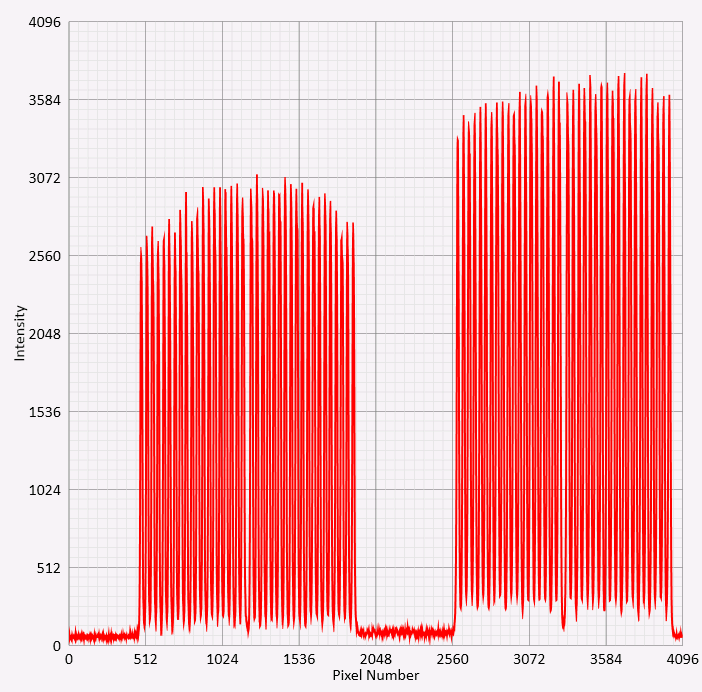
\includegraphics[width=\textwidth]{BRSReadoutScreenPatterns.png}
\section{Signal Processing}
\section{User Interface}

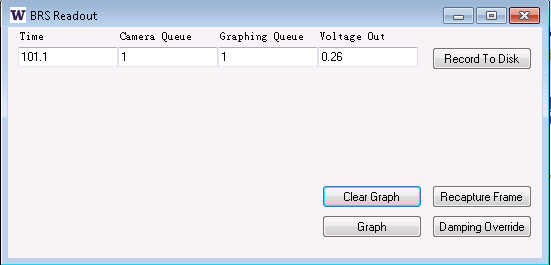
\includegraphics[width=\textwidth]{BRSReadoutScreen.png}\\
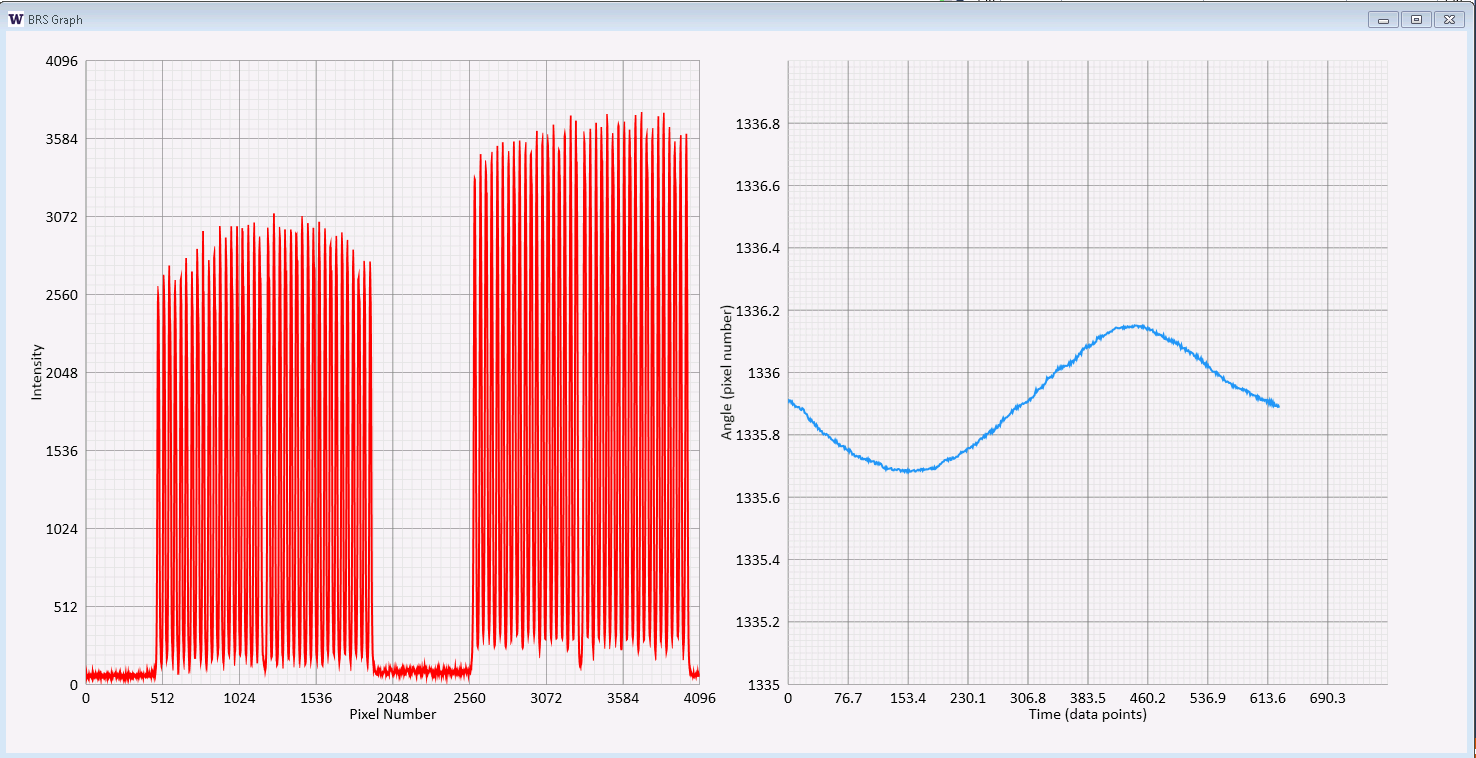
\includegraphics[width=\textwidth]{BRSReadoutScreenGraph.png}

\bibliographystyle{plain}
\bibliography{ReadoutDescription}{}
\end{document}